
During the requirement analysis of the challenge, the general model federation approach remains the foundation of our reflections and modeling intentions. 

First, the federation approach is mainly based on modeling relationships among several models, independently of abstraction levels and model architectures.
The next step in our approach, we try to take into account the reusability of the relationships by identifying the meaning, or semantics, associated with each relationship, in a goal of concept reification with their behavior. The last step is to organize or structure these concepts to improve reusability and extensibility, to create VirtualModels in our Openflexo framework.     

Like any modeling approaches, these different steps could also be achieved in any order. But our goal during the challenge requirement analysis remains to lead to define a FML Virtual Models architecture as a federation of virtualmodels.


~\\
~\\

any disambiguations of the  case  description and assumptions made, any potentially added requirements

quelles hypothèses supplémentaires ? 

+ architecture de la modélisation (ce qui se trouve dans le ppt), le détail se retrouvera dans la section suivante

%Joel commence

% Sylvain
% Joel, je te propose les deux figures suivantes:

\begin{figure}
    \centering
    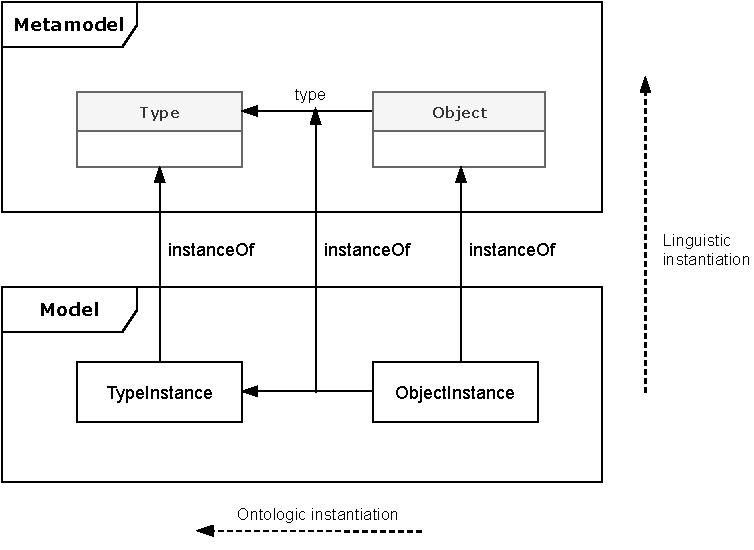
\includegraphics[width=1.0 \columnwidth]{Figures/Instantiation.pdf}
    \caption{Linguistic and ontologic instantiation}
    \label{fig:LinguisticAndOntologicInstantiation}
\end{figure}

\begin{figure}
    \centering
    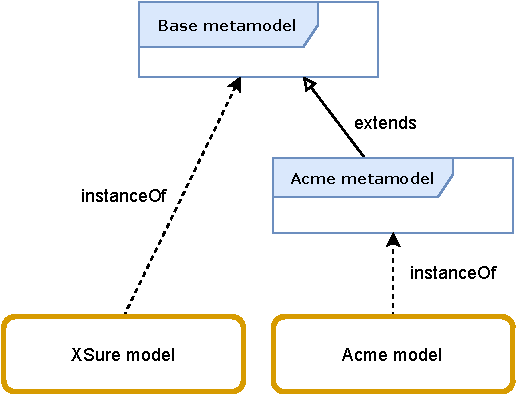
\includegraphics[width=0.7 \columnwidth]{Figures/MultilevelArchitecture.pdf}
    \caption{Multilevel architecture for the Process Challenge}
    \label{fig:MultilevelArchitecture}
\end{figure}


